A cross-correlation measurement between DESI-like LRGs selected from DECaLS imaging and CMB lensing from Planck 2018 is detected at a significance of S/N $= 27.2$ over the range of scales $\ell_{\rm min}=30$ to $\ell_{\rm max}=1000$. In Figure~\ref{fig:snr}, we plot per-multipole and cumulative signal-to-noise ratios for both the galaxy-galaxy and galaxy-convergence spectra, where the signal-to-noise ratio of the $XY$ angular power spectrum at multipole $\ell$ is given by
\begin{equation}
    {\bigg (} \frac{S}{N}{\bigg )}(\ell) = \frac{C_{\ell}^{\rm XY}}{\sigma_{\ell}^{\rm XY}}
\end{equation}
and the cumulative signal-to-noise ratio up to $\ell_{\rm max}$ is
\begin{equation}
    {\bigg (} \frac{S}{N}{\bigg )}(< \ell_{\rm max}) = \sqrt{\sum_{\ell^{\prime}=\ell_{\rm min}}^{\ell_{\rm max}}\frac{(C_{\ell^{\prime}}^{\rm XY})^2}{(\sigma_{\ell^{\prime}}^{\rm XY})^2}}
\end{equation}
The galaxy-galaxy S/N peaks at $\ell \sim 500$ whereas the galaxy-convergence generally decreases over the range of scales considered. We note that the theoretical galaxy-convergence S/N would be expected to peak at $\ell \sim 100$ and fall off at smaller $\ell$; as this is within the regime at which both the pseudo-$C_{\ell}$ framework and the Limber approximation begin to break down, this feature is washed out in the observed S/N.

\begin{figure}
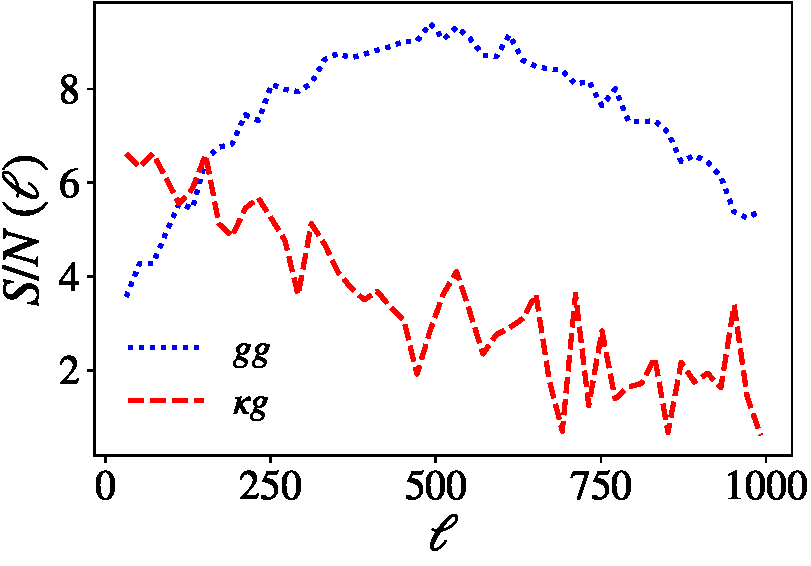
\includegraphics[width=0.9\linewidth]{figures/snr.pdf}
\vspace{1cm}
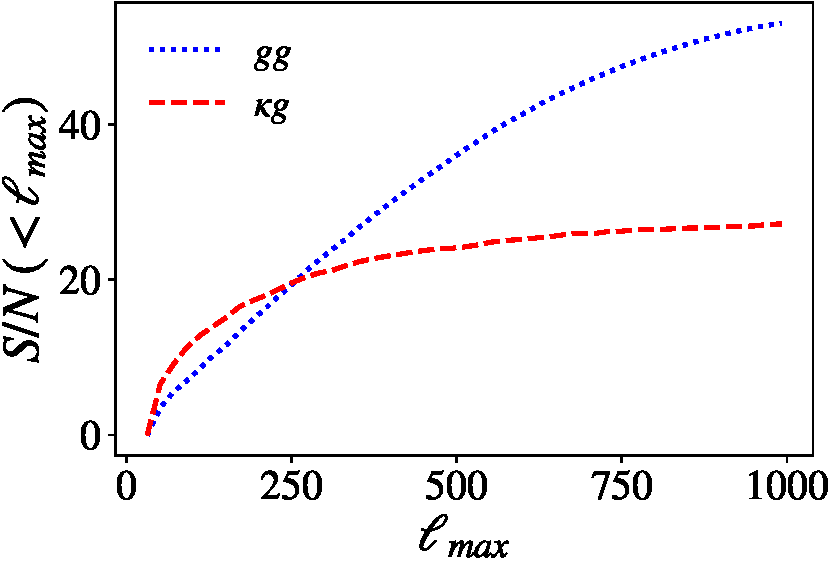
\includegraphics[width=0.9\linewidth]{figures/snr_cum.pdf}
\caption{Per multipole (upper) and cumulative (lower) signal-to-noise ratio for the galaxy-galaxy (blue dotted line) and galaxy-convergence (red dashed line) angular power spectra measurements.}
\label{fig:snr}
\end{figure}

We also compare the cross-spectrum using the baseline MV CMB lensing map versus using the TT-only tSZ-deprojected map. The two curves are shown in the top panel of Figure~\ref{fig:basevdeproj}, and clearly lie well within $1\sigma$ of one another. The fractional difference is shown in the lower panel. Since the error bars on the cross-spectra are generally large, they dominate the errors on the fraction, but as Figure~\ref{fig:basevdeproj} illustrates, the errors associated with tSZ are on the order of a few percent and very subdominant to the overall lensing noise.

\begin{figure}
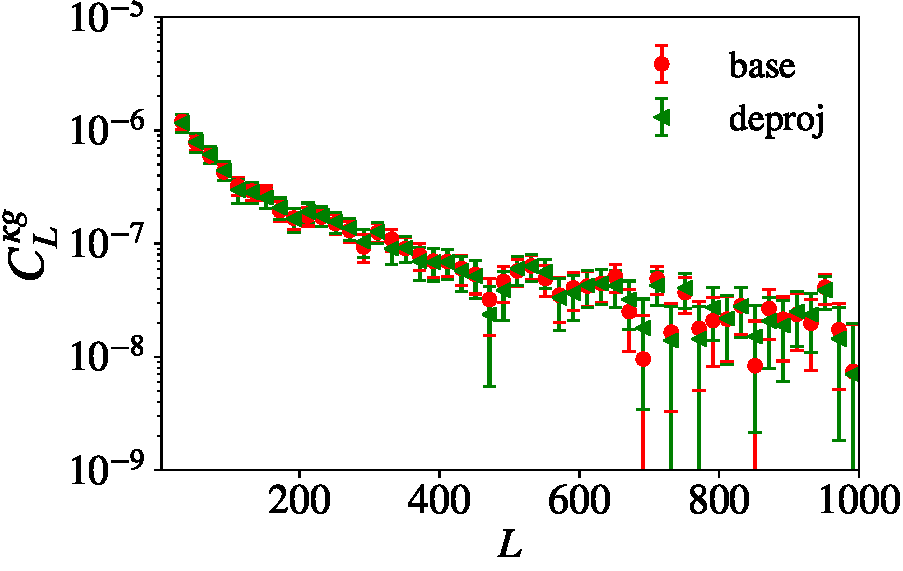
\includegraphics[width=0.9\linewidth]{figures/basevdeproj.pdf}
\vspace{1cm}
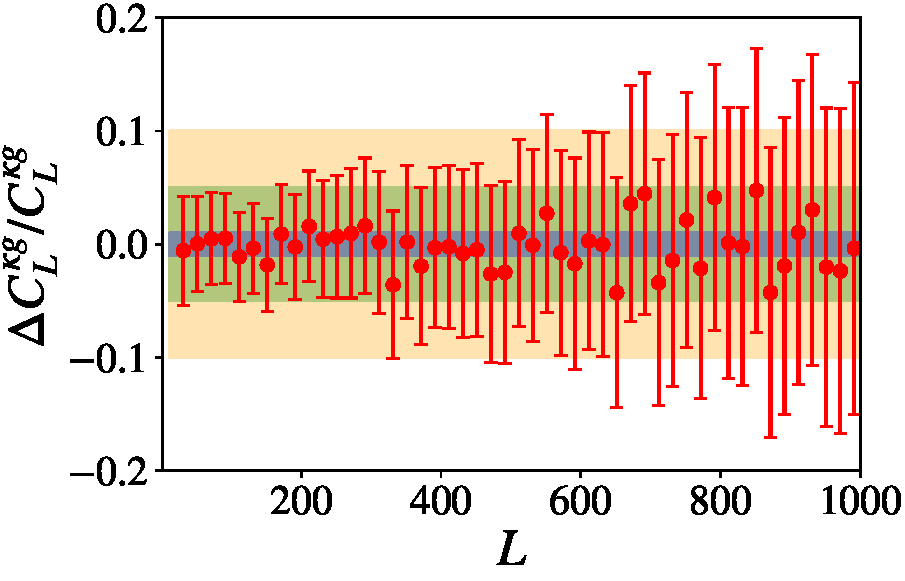
\includegraphics[width=0.9\linewidth]{figures/basevdeproj_frac.pdf}
\caption{Upper: Comparison of observed cross-spectrum $C_{L}^{\kappa g}$ calculated from \texttt{BASE} (red circles) versus \texttt{DEPROJ} (green triangles) lensing maps. Lower: The difference between the two measurements as a fraction of the theoretical prediction, with three bands illustrating 1\%, 5\% and 10\%.}
\label{fig:basevdeproj}
\end{figure}

In the following sub-sections, we present the angular power spectra and interpret them using two different models for the galaxy-galaxy and matter-galaxy 3D power spectra: the HaloFit dark matter power spectrum multiplied by a linear large-scale bias, and a convolutional Lagrangian effective field theory with Lagrangian bias. Additionally, we perform the fits using both photometric- and clustering-derived redshift distributions for the galaxy sample, which not only suggests an estimate of the error associated with uncertainty in the redshift distribution, but also allows us to evaluate the bias at an effective redshift $z \approx 0.68$ in both models and to test the assumption of passive bias evolution. 


\subsection{HaloFit Modeling}\label{sec:results/halofit}
Within a framework for modeling the galaxy-galaxy and matter-galaxy power spectra $P_{\rm gg}(k)$, $P_{\rm mg}(k)$, the observed angular power spectra $C_{\ell}^{\rm gg}$, $C_{\ell}^{\rm \kappa g}$ can constrain cosmological and galaxy bias parameters. A particularly simple and interpretable model is to use the HaloFit \citep{Smith++03} fitting function for the nonlinear dark matter power spectrum, $P_{\rm mm}^{\rm HF}(k)$, and multiply by scale-independent linear biases to obtain the galaxy-galaxy and galaxy-matter power spectra,
\begin{align}
    P_{\rm gg}(k,z) &= b_{\rm gg}(z)^2 P_{\rm mm}^{\rm HF}(k,z) \\
    P_{\rm \kappa g}(k,z) &= b_{\rm \kappa g}(z) P_{\rm mm}^{\rm HF}(k,z)
\end{align}
Differences between $b_{\rm gg}$ and $b_{\rm \kappa g}$ are expected, due in large part to the stochastic contribution arising from the the fact that the galaxy field is a discrete sampling of the underlying dark matter distribution. As such, this stochastic component, which may include scale-dependent and non-Poissonian behavior, affects the galaxy-galaxy auto-spectrum and matter-galaxy cross-spectrum differently.

Using the Boltzmann code \texttt{CLASS} \citep{Blas++11} to calculate the HaloFit dark matter power spectrum for the fiducial Planck 2018 cosmology, we take the photometric $\phi(z)$ and assume a bias evolution $b_{\rm gg}(z), b_{\rm \kappa g}(z) \propto D(z)^{-1}$. We then perform weighted least squares fits of the present day biases. The results are given in Table~\ref{tab:halofit_photo}, with the fits repeated for $\ell_{\rm max} = 200, 400, 600, 800, 1000$. We find that the linear biases are unaffected by the choice of $\ell_{\rm max}$ and that the cross bias $b_{\rm \kappa g}$ is consistently lower than the galaxy bias $b_{\rm gg}$, with the latter agreeing well with DESI survey expectations and the findings of \citealt{Kitanidis++19}.  The lower-than-expected $b_{\rm \kappa g}$ could arise from choosing an incorrect fiducial cosmology (e.g.\ lowering $\Omega_m$ would reduce $b_{\rm \kappa g}$ with only a small impact on $b_{\rm gg}$; see also Hang et al., in prep).  It could also be due to the assumed bias evolution, the assumed form for $\phi(z)$ or limitations of our model.  We shall consider these next.

\begin{table}
\centering
HaloFit Model, Photo $\phi(z)$
\begin{tabular}{c|cc|cc}
\hline
$\ell_{\rm max}$ & $b_{\rm gg}$ & $\chi_{\rm gg}^2 / \text{d.o.f.}$ & $b_{\rm \kappa g}$ & $\chi_{\rm \kappa g}^2 / \text{d.o.f.}$\\
\hline
200 & $1.57 \pm 0.05$ & 0.7 / 8  & $1.27 \pm 0.07$ & 4.2 / 8 \\
400 & $1.63 \pm 0.03$ & 3.4 / 18  & $1.32 \pm 0.06$ & 8.1 / 18  \\
600 & $1.66 \pm 0.02$ & 8.4 / 28  & $1.32 \pm 0.05$ & 12.1 / 28  \\
800 & $1.67 \pm 0.02$ & 9.9 / 38  & $1.32 \pm 0.05$ & 20.9 / 38  \\
\textbf{1000} & \bm{$1.64 \pm 0.02$} & \textbf{30.4 / 48}  & \bm{$1.32 \pm 0.05$} & \textbf{26.8 / 48} \\
\hline
\end{tabular}
\caption{Fitting linear bias from the observed $C_{\ell}^{\rm gg}$, $C_{\ell}^{\rm \kappa g}$ up to different $\ell_{\rm max}$ using the HaloFit model for the nonlinear dark matter power spectrum, photometric $\phi(z)$, and the assumption $b(z) \propto D(z)^{-1}$.}
\label{tab:halofit_photo}
\end{table}

\begin{figure}
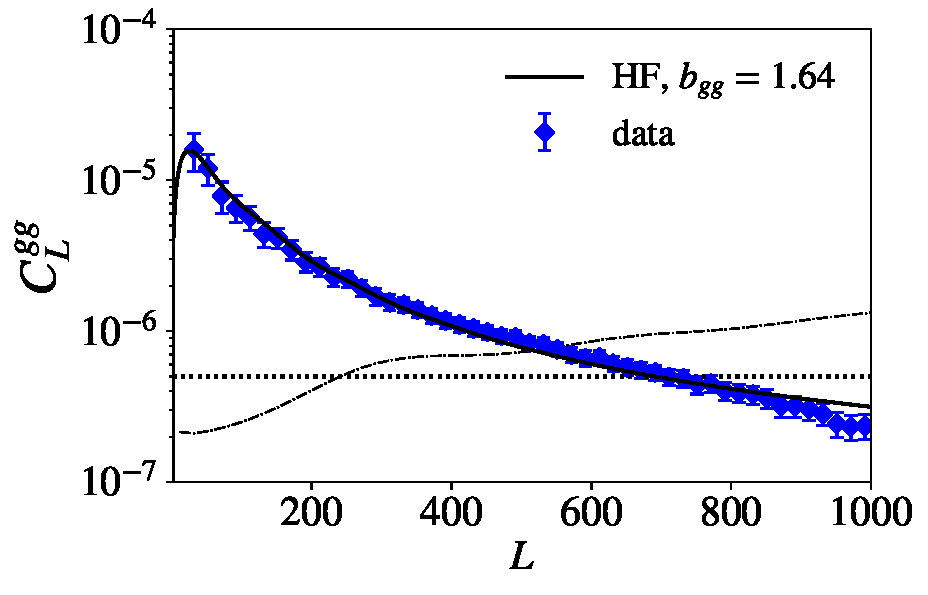
\includegraphics[width=\linewidth]{figures/cl_gg_hf.pdf}
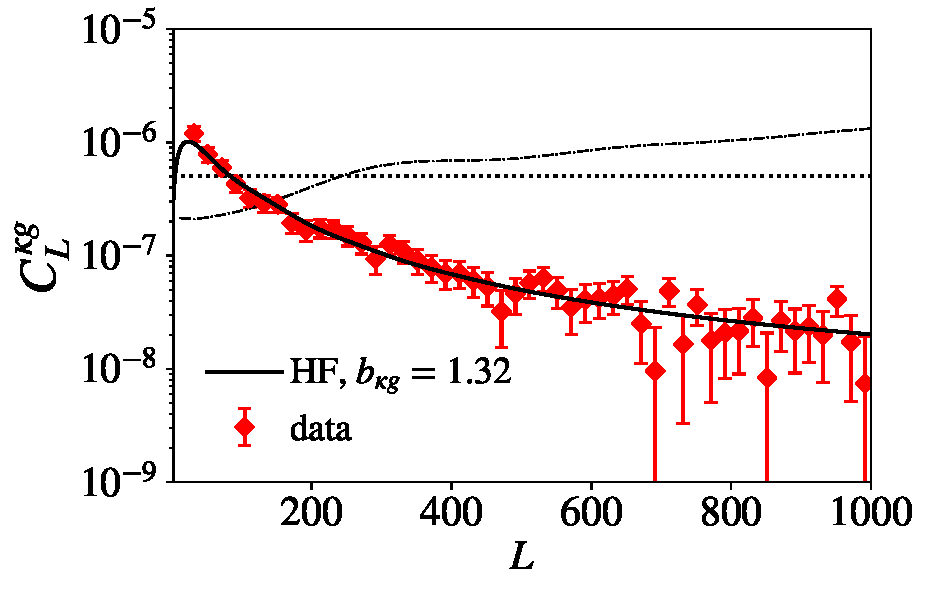
\includegraphics[width=\linewidth]{figures/cl_kg_hf.pdf}
\caption{The observed galaxy-galaxy (upper plot, blue diamonds) and galaxy-convergence (lower plot, red diamonds) angular power spectra, after subtracting noise and correcting for magnification bias. Solid lines correspond to the the theoretical predictions using a HaloFit matter power spectrum and the best fit linear biases from Table~\ref{tab:halofit_photo}. The dotted horizontal line is the galaxy shot noise floor, and the dashed black curve is the lensing noise.}
\label{fig:cl_halofit}
\end{figure}

We then repeat the same measurement using the clustering-derived $\phi(z)$ discussed in Section~\ref{sec:dndz_pipe}, again finding that the choice of $\ell_{\rm max}$ has negligible impact. The results, given in Table~\ref{tab:halofit_clustering}, show that uncertainty in the redshift distribution causes a difference in the derived galaxy bias parameters of $\sigma_{b_{\rm gg}} = 0.08$. By contrast, the cross bias is extremely stable with respect to changes in the redshift distribution, not changing at all when the redshift distribution is changed from the photometric estimate to the clustering estimate; this may be explained by the fact that the cross-spectrum only depends on one factor of $\phi(z)$ while the auto-spectrum requires $\phi^2(z)$.

Another advantage of using the clustering-based $\phi(z)$ is the ability to extract a galaxy redshift kernel with bias evolution baked in, rather than assuming a parametric form e.g. $b(z) \propto D(z)^{-1}$. As discussed in Section~\ref{sec:dndz_pipe/q}, this type of modeling allows us to constrain $b_{\rm eff} \approx b(z_{\rm eff})$ rather than the present day bias. We find the results, given in Table~\ref{tab:halofit_clustering_noevo}, to be in perfect agreement with the results of Table~\ref{tab:halofit_clustering} under the assumption $b(z) \propto D(z)^{-1}$ used in the latter, giving for instance $b_{\rm gg}= 1.56 \pm 0.01$ and $b_{\rm \kappa g}= 1.31 \pm 0.05$ for the $\ell_{\rm max} = 1000$ case. 

\begin{table}
\centering
HaloFit Model, Clustering $\phi(z)$
\begin{tabular}{c|cc|cc}
\hline
$\ell_{\rm max}$ & $b_{\rm gg}$ & $\chi_{\rm gg}^2 / \text{d.o.f.}$ & $b_{\rm \kappa g}$ & $\chi_{\rm \kappa g}^2 / \text{d.o.f.}$\\
\hline
200 & $1.50 \pm 0.05$ & 0.8 / 8  & $1.27 \pm 0.07$ & 4.0 / 8 \\
400 & $1.55 \pm 0.03$ & 3.4 / 18  & $1.32 \pm 0.06$ & 8.0 / 18  \\
600 & $1.59 \pm 0.02$ & 8.7 / 28  & $1.32 \pm 0.05$ & 11.9 / 28  \\
800 & $1.59 \pm 0.02$ & 10.2 / 38  & $1.32 \pm 0.05$ & 20.8 / 38  \\
\textbf{1000} & \bm{$1.56 \pm 0.01$} & \textbf{29.9 / 48}  & \bm{$1.32 \pm 0.05$} & \textbf{26.7 / 48} \\
\hline
\end{tabular}
\caption{Fitting linear bias from the observed $C_{\ell}^{\rm gg}$, $C_{\ell}^{\rm \kappa g}$ up to different $\ell_{\rm max}$ using the HaloFit model for the nonlinear dark matter power spectrum, clustering $\phi(z)$, and the assumption $b(z) \propto D(z)^{-1}$.}
\label{tab:halofit_clustering}
\end{table}

\begin{table}
\centering
HaloFit Model, Clustering $b(z)\phi(z)$
\begin{tabular}{c|cc|cc}
\hline
$\ell_{\rm max}$ & $b^{\rm eff}_{\rm gg}$ & $\chi_{\rm gg}^2 / \text{d.o.f.}$ & $b^{\rm eff}_{\rm \kappa g}$ & $\chi_{\rm \kappa g}^2 / \text{d.o.f.}$\\
\hline
200 & $2.14 \pm 0.07$ & 0.8 / 8  & $1.80 \pm 0.10$ & 4.0 / 8 \\
400 & $2.21 \pm 0.04$ & 3.4 / 18  & $1.89 \pm 0.08$ & 8.0 / 18  \\
600 & $2.26 \pm 0.03$ & 8.7 / 28  & $1.88 \pm 0.08$ & 12.0 / 28  \\
800 & $2.27 \pm 0.02$ & 10.2 / 38  & $1.88 \pm 0.07$ & 20.8 / 38  \\
\textbf{1000} & \bm{$2.23 \pm 0.02$} & \textbf{29.9 / 48}  & \bm{$1.88 \pm 0.07$} & \textbf{26.7 / 48} \\
\hline
\end{tabular}
\caption{Fitting effective bias $b_{\rm eff} \approx b(z_{\rm eff} = 0.68)$ from the observed $C_{\ell}^{\rm gg}$, $C_{\ell}^{\rm \kappa g}$ up to different $\ell_{\rm max}$ using the HaloFit model for the nonlinear dark matter power spectrum, clustering $b(z)\phi(z)$ (normalized), and no assumptions regarding the shape of the bias evolution.}
\label{tab:halofit_clustering_noevo}
\end{table}

\subsection{Perturbation Theory Modelling}\label{sec:results/lpt}
We next apply an analytic model that allows more nuance in the handling of bias. Higher order perturbation theory is a natural approach considering that the cross-correlation is most sensitive to structure at large scales, as shown in see Figure~\ref{fig:snr}. We use a Lagrangian bias model and the convolution Lagrangian effective field theory (hereafter CLEFT) outlined in \citealt{Vlah++16} and the references contained therein. Under this formalism, the matter-galaxy and galaxy-galaxy power spectra are (see e.g.\ Equation 2.7 from \citealt{Modi++17} and Equation B.2 from \citealt{Vlah++16}):
\begin{align}\label{eqn:lpt1}
    P_{\rm mg} &= (1-\frac{\alpha_{\times}k^2}{2})P_{\rm Z} + P_{\rm 1L} + \frac{b_1}{2}P_{\rm b_1} + \frac{b_2}{2}P_{\rm b_2} \\
    \label{eqn:lpt2}
    P_{\rm gg} &= (1-\frac{\alpha_{a}k^2}{2})P_{\rm Z} + P_{\rm 1L} + b_1 P_{\rm b_1} + b_2 P_{\rm b_2} + \\
    & \hspace{0.35cm} b_1 b_2 P_{\rm b_1 b_2}  + b_1^2 P_{\rm b_1^2} + b_2^2 P_{\rm b_2^2} \nonumber
%    & \hspace{0.3cm} + b_{s^{2}} P_{\rm b_{s^{2}}} + b_1 b_{s^{2}} P_{\rm b_1 b_{s^{2}}} \nonumber \\
%    & \hspace{0.3cm}  + b_2 b_{s^{2}} P_{\rm b_2 b_{s^{2}}} + b_{s^{2}}^2 P_{\rm (b_{s^{2}})^2} \nonumber
\end{align}
where we have dropped the terms corresponding to shear bias as we find they mainly affect scales $\ell > 1000$. Here, $P_{\rm Z}$ and $P_{\rm 1L}$ are the Zeldovich and 1-loop dark matter contributions (see e.g. \citealt{Vlah++15}), $b_1$ and $b_2$ are the Lagrangian bias parameters for the galaxy sample, and the effective field theory terms $\alpha_{\times}$ and $\alpha_a$ (which are not necessarily the same) are free parameters encapsulating the small-scale physics not modeled by Lagrangian perturbation theory.

Under the CLEFT formalism, the power spectrum contributions $P_{\rm Z}$, $P_{\rm 1L}$, $P_{\rm b_1}$, $P_{\rm b_2}$, etc. can be computed analytically and combined with the free parameters $\alpha_{\times}, \alpha_a, b_1, b_2$. With these additional degrees of freedom, CLEFT provides a more flexible model than the phenomenological approach of Section~\ref{sec:results/halofit}, and allows us to fit the cross-spectrum and galaxy auto-spectrum simultaneously.

We use a version of the public code \texttt{velocileptors}\footnote{\url{https://github.com/sfschen/velocileptors}} \citep{velocileptors} to calculate the power spectrum terms and the MCMC likelihood estimator \texttt{emcee}\footnote{\url{https://github.com/dfm/emcee}} \citep{emcee} to optimize our model parameters. 
%In addition to the six free parameters in Equations~\ref{eqn:lpt1} and \ref{eqn:lpt2} representing the galaxy-halo connection, we also wish to constrain the cosmological parameter $\sigma_8$; with galaxy clustering alone, there is significant degeneracy between $\sigma_8$ and galaxy bias, but this degeneracy is broken by including the cross-correlation with CMB lensing convergence. 
To reduce model expense, we evaluate the power spectrum terms at a single effective redshift,
\begin{equation}
    z_{\rm eff}^{XY} = \frac{\int d\chi \ z \ W^{X}(\chi)W^{Y}(\chi)/\chi^2}{\int d\chi \ W^{X}(\chi)W^{Y}(\chi)/\chi^2}
\end{equation}
which is $z_{\rm eff} = 0.67$ for $\kappa g$ and $z_{\rm eff} = 0.68$ for $gg$\footnote{To jointly fit the auto- and cross-spectrum, we assume $z_{\rm eff} = 0.68$ for both.}. Given the narrow redshift distribution and likely passive bias evolution of our galaxy sample, this substitution should not affect the $C_{\ell}$'s significantly \citep{Modi++17}, and we confirm that the overall impact on the scales of interest is sub-percent level. Additionally, this allows us to more easily interpret the Lagrangian bias parameters as being also evaluated at the effective redshift. We use the photometric redshift distribution to eliminate the need to assume a shape for the bias evolution.

We perform a joint fit on both the galaxy-galaxy auto-spectrum and galaxy-convergence cross-spectrum using a simple Gaussian likelihood function:
\begin{align}
    \mathcal{L}(d|\vartheta) \propto \exp {\Big \{ }-\frac{1}{2}(\hat{C}(\vartheta) - {C}) \ {\Sigma}^{-1} \ (\hat{C}(\vartheta) - {C})^{\rm T}{\Big \} }
\end{align}
The vectors $C$ and $\hat{C}(\vartheta)$ are, respectively, the observed and predicted angular power spectra, with the auto- and cross-spectrum measurements joined together as
\begin{align}
    {C_{L}} &= (C^{\rm \kappa g}_{L}, C^{\rm gg}_{L})
\end{align}
for each bandwidth bin $L$. The covariance matrix is created from the four constituent covariance matrices,
\begin{align}
    {\Sigma_{LL^{\prime}}} &= 
    \begin{pmatrix}
    \Sigma^{\rm \kappa g}_{LL^{\prime}} & (\Sigma^{\kappa g - gg}_{LL^{\prime}})^{\rm T} \\
    \Sigma^{\kappa g - gg}_{LL^{\prime}} & \Sigma^{\rm gg}_{LL^{\prime}}
    \end{pmatrix}
\end{align}
The covariance matrices $\Sigma^{\rm \kappa g}_{LL^{\prime}}$ and $\Sigma^{\rm gg}_{LL^{\prime}}$ are given by Equations~\ref{eq:cov_gen}. Similarly, the Gaussian part of the covariance between the auto-spectrum and cross-spectrum measurements is given by
\begin{align}
    \Sigma^{\kappa g - gg}_{LL^{\prime}} &=
     (\sigma_{L}^{\kappa g - gg})^2 \delta_{L L^{\prime}}
\end{align}
where
\begin{align}
    \frac{1}{(\sigma_{L}^{\kappa g - gg})^2} &= \frac{1}{\Delta \ell} \sum_{\ell \in L} \frac{1}{(\sigma_{\ell}^{\kappa g - gg})^2} \\
    (\sigma_{\ell}^{\kappa g - gg})^2 &= \frac{[2 C^{\rm \kappa g}_{\ell}(C^{\rm gg}_{\ell} + N^{\rm gg}_{\ell}) ]_{\rm th}}{f_{\rm sky}(2\ell + 1)}\frac{w_4}{w_2^2}
\end{align}

We use flat priors for the four model parameters, and additionally impose a loose Gaussian prior on $b_2$ centered on the peak-background split prediction for a given $b_1$. The results of the MCMC analysis are listed in Table~\ref{tab:lpt_mcmc} for $\ell_{\rm max} = 200$, 400, 600, 800 and 1000.  Although the higher $\ell_{\rm max}$ are formally larger than the regime of validity of perturbation theory ($\ell_{\rm max}\lesssim 500$) we nonetheless find that the best fit parameters remain stable within error bars and the inclusion of the higher $\ell$ data helps to fix the EFT counter terms. The corner plots visualizing the 1D and 2D posterior distributions are shown in Figure~\ref{fig:lptmcmc}, and the resulting theory predictions are plotted against the binned data in Figure~\ref{fig:cl_lptfit}, both for the $\ell_{\rm max} = 1000$ case. The values and errors are based on  16th, 50th, and 84th percentiles of the posterior distributions. The model is able to constrain $b_1$ very well, and provides a more flexible fit to the shape of the data.

\begin{table*}
\centering
CLEFT Model, Photo $\phi(z)$ \\
\begin{tabular}{ccccccc}
%\begin{tabular}{ p{0.9cm} | p{1.6cm} | p{1.3cm} | p{1.1cm} | p{1.1cm} | p{1.1cm}}
\hline
& & \multicolumn{5}{c}{Posterior} \\
\cmidrule{3-7}
Parameter & Prior & $\ell_{\rm max} = 200$ & $\ell_{\rm max} = 400$ & \bm{$\ell_{\rm max} = 600$} & $\ell_{\rm max} = 800$ & $\ell_{\rm max} = 1000$ \\
\hline
%$\sigma_8$ & $\in[0.5,1]$ & $A^{+B}_{-C}$ \\
$b_1$ & $\in[0.5, 1.5]$ & $1.33^{+0.05}_{-0.05}$ & $1.30^{+0.05}_{-0.06}$ & \bm{$1.31^{+0.05}_{-0.05}$} & $1.32^{+0.04}_{-0.04}$ & $1.33^{+0.04}_{-0.04}$ \vspace{0.15cm} \\
$b_2$ & $ \in[-1, 2] $, $ \propto\mathcal{N}\big{(} \tilde{b}_2, 0.3 \big{)} $  & $0.529^{+0.292}_{-0.318}$ & $0.192^{+0.283}_{-0.316}$ & \bm{$0.347^{+0.291}_{-0.332}$} & $0.352^{+0.294}_{-0.305}$ & $0.514^{+0.255}_{-0.283}$ \vspace{0.15cm} \\
%      & $ \propto\mathcal{N}\big{(} \tilde{b}_2, 0.3 \big{)}$ & \\
%$b_{s^2}$ & $\in[?,?]$ & $A^{+B}_{-C}$ & x/y  \\
$\alpha_{\times}$ & $\in[-100,100]$ & $94.42^{+4.09}_{-8.49}$ & $87.73^{+8.64}_{-12.78}$ & \bm{$50.51^{+9.90}_{-10.91}$} & $28.84^{+7.59}_{-7.60}$ & $19.74^{+5.94}_{-6.13}$  \vspace{0.15cm} \\
$\alpha_a$ & $\in[-100,100]$ & $-77.88^{+33.45}_{-16.25}$ & $20.68^{+50.71}_{-55.44}$ & \bm{$21.33^{+38.25}_{-36.01}$} & $14.28^{+24.73}_{-24.88}$ & $33.23^{+17.54}_{-18.25}$ \vspace{0.15cm} \\
%$s_a$ & $\in[0.5 \frac{1}{\bar{n}},1.5 \frac{1}{\bar{n}}]$ & $A^{+B}_{-C}$ \\
\hline
\end{tabular}
\caption{Fits of the perturbation theory based model to $C_\ell^{gg}$ and $C_\ell^{\kappa g}$ as a function of $\ell_{\rm max}$.  The second column lists the priors used for the LPT model parameters, while the third column is the medians and $1\sigma$ confidence intervals based on the 16th and 84th percentiles of the posterior distributions. All priors are flat except for the prior on $b_2$, which is a Gaussian loosely centered at the peak-background split prediction for a given $b_1$.}
\label{tab:lpt_mcmc}
\end{table*}

\begin{figure}
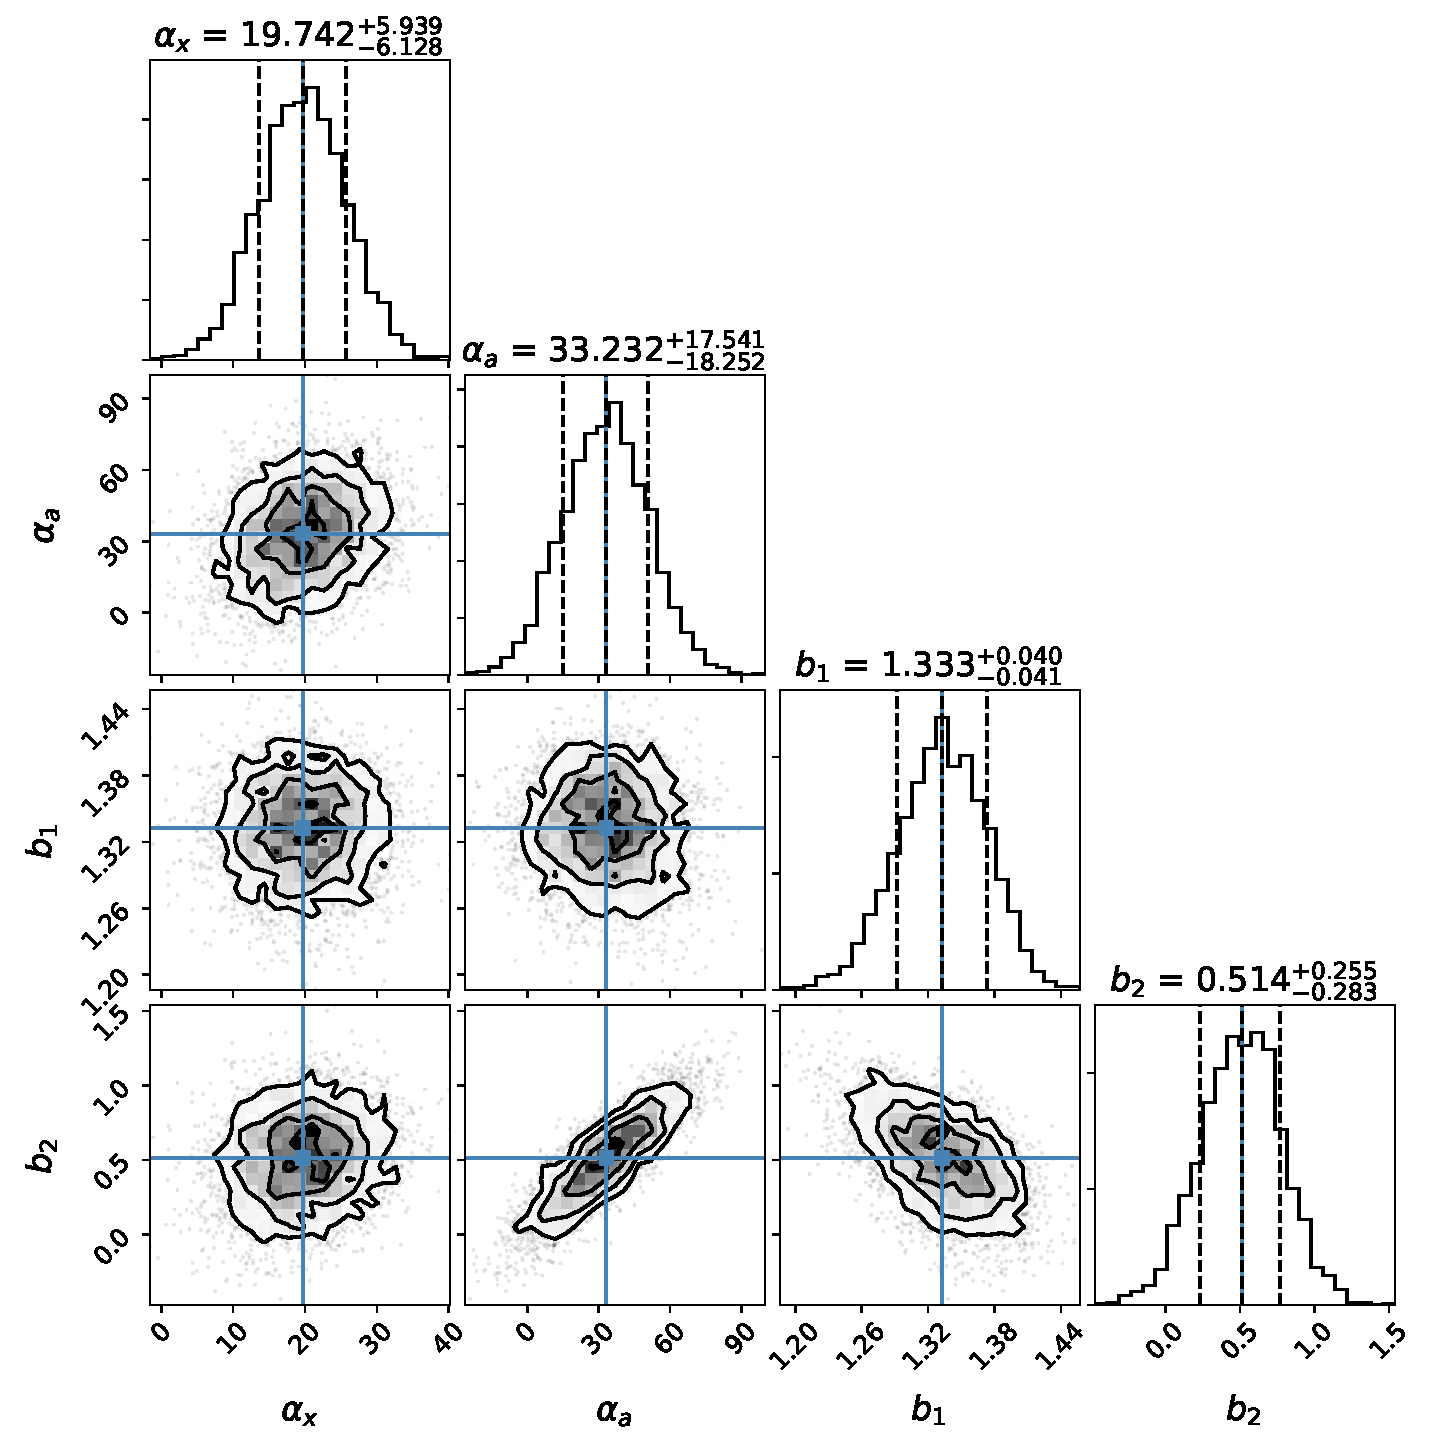
\includegraphics[width=\linewidth,trim={0.4cm 0.2cm 0.2cm 0.2cm},clip]{figures/corner_plot.pdf}
\caption{Marginalized 1D and 2D posterior probability distributions of the parameters. Vertical lines are median values.}
\label{fig:lptmcmc}
\end{figure}

\begin{figure}
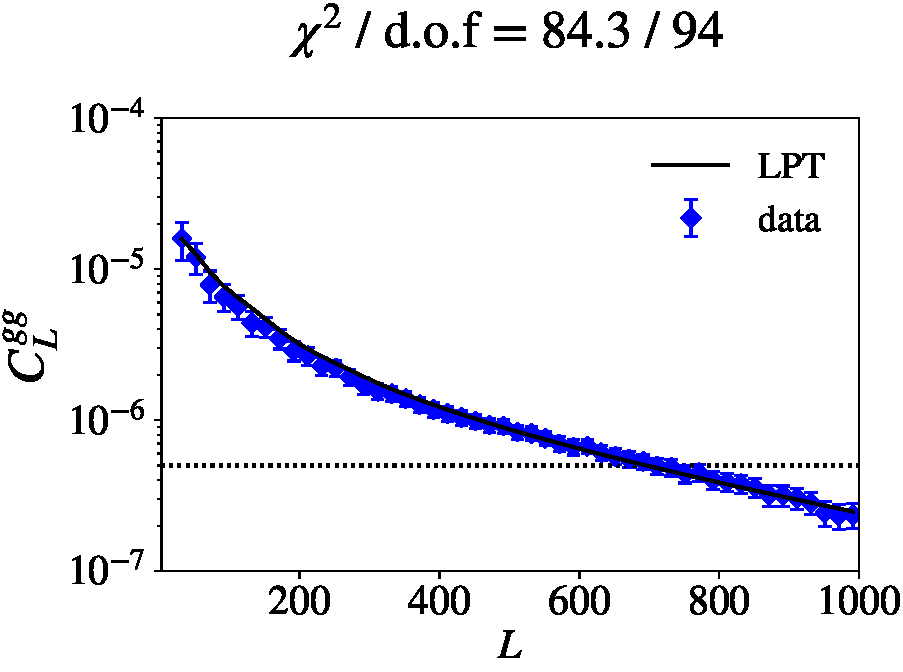
\includegraphics[width=\linewidth]{figures/cl_gg_lpt.pdf}
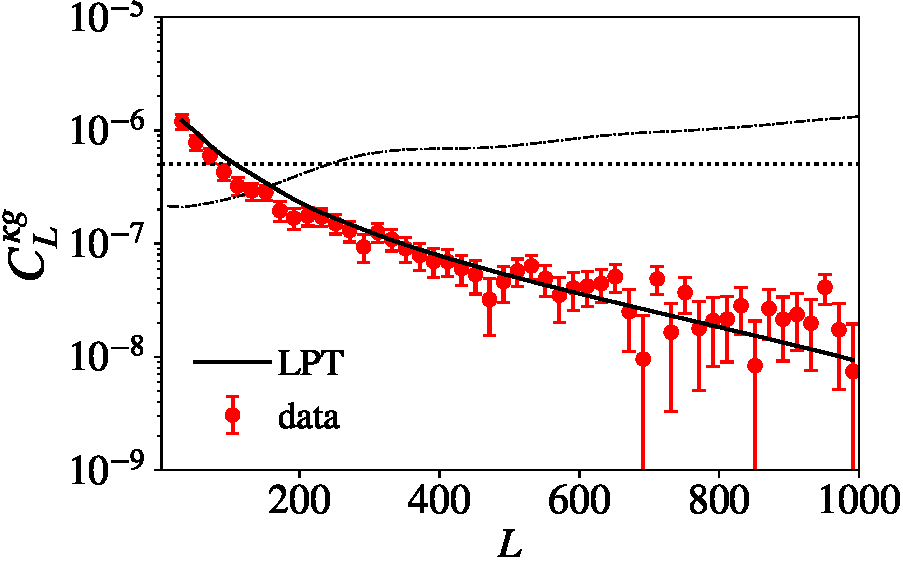
\includegraphics[width=\linewidth]{figures/cl_kg_lpt.pdf}
\caption{The observed galaxy-galaxy (upper plot, blue diamonds) and galaxy-convergence (lower plot, red diamonds) angular power spectra, after subtracting noise and correcting for magnification bias. Solid lines correspond to the predictions from the CLEFT perturbation theory framework using MCMC fitted parameters for $\ell_{\rm max}=1000$ (Table~\ref{tab:lpt_mcmc}). The dotted horizontal line is the galaxy shot noise floor, and the dashed black curve is the lensing noise.}
\label{fig:cl_lptfit}
\end{figure}

We can compare the Lagrangian $b_1$ to the Eulerian bias found in the previous section,
\begin{align}
    b(z_{\rm eff}) &= 1 + b_1(z_{\rm eff}) \\
    &= b(0)/D(z_{\rm eff})
\end{align}
For $z_{\rm eff} = 0.68$, the best fit $b_1 = 1.31$ corresponds to $b(0) = 1.63$, in excellent agreement with the result from our HaloFit model using the photometric redshift distribution. Furthermore, after accounting for the uncertainty associated with photometric versus clustering redshift distributions $\sigma_{b_{\rm gg}} = 0.08$, the effective bias from the perturbation theory model is consistent with the effective bias measured using the clustering $b(z)\phi(z)$ (Table~\ref{tab:halofit_clustering_noevo}). Thus, these two models show excellent consistency with each other, and both are consistent with the assumed bias evolution model.  The LPT-based model provides a statistically acceptable fit to both $C_\ell^{\rm gg}$ and $C_\ell^{\rm \kappa g}$ for our fiducial cosmology, however if one artificially introduces an additional degree of freedom that scales the amplitude of $C_\ell^{\rm \kappa g}$ we find an even better fit is obtained when the model prediction is lowered by 10-20\%.  This is similar to the lower $b_{\rm \kappa g}$ preferred by our HaloFit model, compared to $b_{\rm gg}$.


\subsection{Bandpower covariance}\label{sec:results/discussion}

In order to evaluate whether correlated bandpower bins contribute to low reduced chi-square in the fits, we repeat the full analysis using bandpower bins of $\Delta \ell = 100$ instead of 20. The recovered bias parameters remain the same, and the reduced chi-square of the fits do not appreciably change. Since $\chi^2$ / d.o.f.\ should be preserved under changes in binning scheme if the bins are uncorrelated, we consider this sufficient evidence that our bins of $\Delta \ell = 20$ are largely uncorrelated. As another test, we also performed the fits using $\ell_{\rm min} = 100$ instead of $\ell_{\rm min} = 30$ and again found that the results and goodness-of-fit remained stable suggesting that large scales are not driving our fitting results.

%\subsection{HOD Modelling}
%\subsection{Basic formalism}

\subsection{N-body simulation and halo catalog}

\subsection{HOD model and synthetic galaxy catalogs}

We use the HOD model of Zheng et al. (2005). In this framework, it is assumed that central galaxies sit at the precise centers of their host halos and that the spatial distributions of satellite galaxies follow unbiased NFW profiles (Navarro et al. 1997). The occupation statistics of central galaxies are described by a Bernoulli distribution (since a halo can either have none or one central galaxies), with the first moment given by a step-like function parameterized as
\begin{align}
    \langle N_{\rm cen} | M \rangle &= \frac{1}{2}{\bigg [}1 + \text{erf}{\bigg(}\frac{\log M - \log M_{\rm min}}{\sigma_{\log M}}{\bigg)}{\bigg ]} \label{eqn:hod_cen}
\end{align}
Here, $M_{\rm min}$ is the minimum mass threshold above which a halo can host a central galaxy, while $\sigma_{\log M}$ represents the scatter in the relation between the virial mass of the dark matter halo and the baryonic mass of the central galaxy and thus controls the width of the transition from $\langle N_{\rm cen} \rangle = 0$ to $\langle N_{\rm cen} \rangle = 1$. 

The occupation statistics of satellite galaxies are roughly Poisson, with the first moment given by a truncated power law parameterized as 
\begin{align}
    \langle N_{\rm sat} | M \rangle &= {\bigg (}\frac{M - M_0}{M_1}{\bigg )}^{\alpha}\vartheta(M - M_0) \label{eqn:hod_sat}
\end{align}
where $\alpha$ is the slope, $M_0$ is the low-mass cutoff, and $M_1$ is the characteristic mass at which $\langle N_{\rm sat} \rangle$ begins to follow a power law. The Heaviside function enforces that no satellite galaxies reside in halos with $M < M_0$.

\subsection{Bayesian likelihood analysis}

\begin{align}
    \ln{\mathcal{L}(d|\vartheta)} = -\frac{1}{2} \sum_{\ell\ell^{'}} \ (C_{\ell}^{\rm th}(\vartheta) - C_{\ell}^{\rm d}) \ \text{Cov}(C_{\ell},C_{\ell^{'}})^{-1} \ (C_{\ell^{'}}^{\rm th}(\vartheta) - C_{\ell^{'}}^{\rm d})
\end{align}
where $C_{\ell}^{\rm th}(\vartheta)$ is the theoretical angular power spectrum for a given set of HOD parameters $\vartheta$, $C_{\ell}^{\rm d}$ is the observed angular power spectrum from the data, and $\text{Cov}(C_{\ell},C_{\ell^{'}})$ is the covariance matrix. Note that we only compute the Gaussian (``disconnected'' part) covariance matrix, as this is the dominant contribution on large scales.

\subsection{Results}

\begin{table}
\centering
\begin{tabular}{cllc} 
Parameter & Prior  & Posterior & $\chi^2 / \text{d.o.f.}$\\
\hline
$\log{(M_{\rm min} / M_{\odot})}$ & $\in[9,16]$ & $A^{+B}_{-C}$ & x/y  \\
$\sigma_{\log{M}}$ & $\in[0.001, 2]$ & $A^{+B}_{-C}$ & x/y  \\
$\alpha$ & $ \in[0,2]$ & $A^{+B}_{-C}$ & x/y  \\
$\log{(M_{0} / M_{\odot})}$ & $\in[9,16]$ & $A^{+B}_{-C}$ & x/y  \\
$\log{(M_{1} / M_{\odot})}$ & $\in[9,16]$ & $A^{+B}_{-C}$ & x/y \\
\hline
\end{tabular}
\caption{The second column lists the flat prior ranges used for the HOD model parameters, while the third column is the medians and $1\sigma$ confidence intervals of the posterior distributions. The last column describes the goodness-of-fit.}
\label{tab:hod_mcmc}
\end{table}

